\chapter{LIMEFS}
\index{LIMEFS}

\section{Introduction}

The LIMEFS filesystem contains a few distinctive characteristics:

\begin{itemize}
\item In-memory meta data \\
All \wi{meta data} used is in memory and stored consecutively on disk. This ensures fast updating, with few I/O operations. Most administration is built on-the-fly during mount time.
\item Few files/inodes \\
This filesystem is designed to store a few very large files. This makes a larger-than-normal data block size desirable.
\item Extent structure \\
Extents\footnote{An \wi{extent} is an ( offset, length ) tuple} are used to maintain data block administration.
\item Disk block size \\
The filesystem can use an user-defined block size, which is used for all I/O requests. This allows for good performance.
\item Inodes belong to directories \\
A directory is not a list of inodes residing in it. Each inode knows to which directory it belongs. Since all meta data is stored in-memory, this has barely any performance constraints.
\end{itemize}

The LIMEFS filesystem is designed to provide predictable performance.

Realtime I/O scheduling is not part of the filesystem. In order to have guaranteed disk I/O performance, the \wi{ABISS} framework is used. This framework can provide realtime I/O performance based on the application's wishes. ABISS itself is a separate project, more information can be found at \cite{ABISS}.

\section{Overview}

If we view a disk as an one-dimensional array of sectors, the next figure displays the on-disk structure:

\begin{figure}[h]
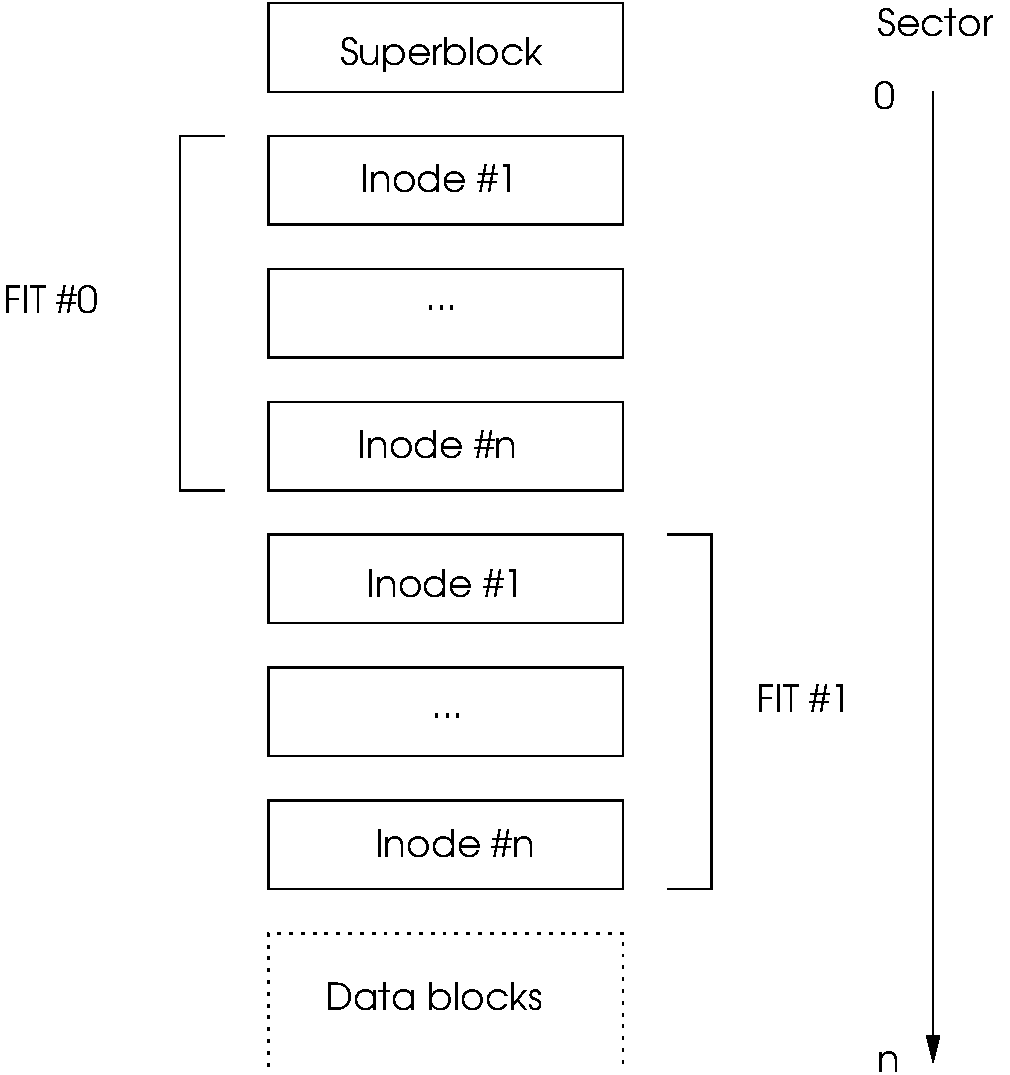
\includegraphics[height=8cm]{disk-layout}
\caption{On-disk structure of the filesystem}
\end{figure}

\begin{itemize}
\item Superblock \\
This is the very first filesystem structure. It contains read-only information needed to mount the filesystem.
\item File Information Table \\
The File Information Table, FIT, contains the inodes.
\item Data blocks \\
Space where the file data resides.
\end{itemize}

These structures will be explained in the next paragraphs.

\section{Superblock}
\label{superblock}

The \wi{superblock} contains a magic value used to identify the filesystem, as well as information used for mounting. The superblock is \emph{readonly}, and all values in it are copied to memory. This copy is used as long as the filesystem is mounted.

\index{struct!lime\_superblock}
\begin{verbatim}
struct lime_superblock {
 uint32_t sb_magic;
 uint32_t sb_version;
 uint32_t sb_diskBlockSize;
 uint32_t sb_dataBlockSize;
 uint64_t sb_numDiskBlocks;
 uint32_t sb_inodeSize;
 uint32_t sb_numInodes;
};
\end{verbatim}

\begin{tabularx}{\textwidth}{|l|X|}
\hline
sb\_magic&Magic value used for identification \texttt{LIME\_SB\_MAGIC (0xFC492B42)}\\
\hline
sb\_version&Current version number, \texttt{LIME\_SB\_VERSION (0x0001)}\\
\hline
sb\_diskBlockSize&Size of a disk block, in bytes. Due to Linux constrains, this may not exceed a page size (4KB on x86)\\
\hline
sb\_dataBlockSize&Size of a data block, in bytes. This must be a multiple of sb\_diskBlockSize.\\
\hline
sb\_numDiskBlocks&Total number of blocks on the disk (in sb\_diskBlockSize byte blocks)\\
\hline
sb\_inodeSize&Size of a single inode structure. Should be \texttt{1024} for version 1\\
\hline
sb\_numInodes&Total number of inodes on the filesystem, including reserved\footnote{reserved inodes are the root and checkpoint inodes} ones\\
\hline
\end{tabularx}

The next page will show an overview of the calculations with their corresponding place on the disk.

\newpage

Based on these values, calculations are made for often-used values:

\begin{displaymath}
fit\_in\_diskblocks = \frac{sbInodeSize * sbNumInodes + sbDiskBlockSize - 1}{sbDiskBlockSize}
\end{displaymath}
\begin{displaymath}
firstDataBlock = \frac{(1 + NUM\_FITS * fit\_in\_diskblocks) + \frac{sbDataBlockSize}{sbDiskBlockSize} - 1}{\frac{sbDataBlockSize}{sbDiskBlockSize}}
\end{displaymath}
\begin{displaymath}
numDataBlocks = \frac{sb\_numDiskBlocks}{\frac{sbDataBlockSize}{sbDiskBlockSize}} - firstDataBlock 
\end{displaymath}
\begin{displaymath}
fitOffset(n) = 1 + (n * fit\_in\_diskblocks)
\end{displaymath}

Graphically, this gives:

\begin{figure}[h]
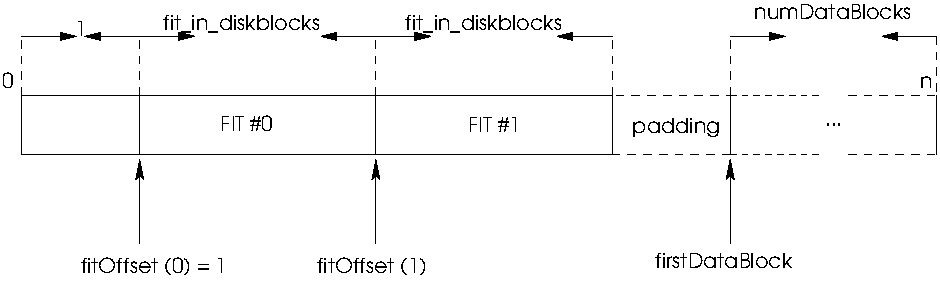
\includegraphics[width=12cm]{calc}
\caption{Internal offsets of on-disk structures}
\end{figure}

\section{File Information Table}
\label{fit}

A \wi{File Information Table} is an array of all inodes on the disk, and therefore spans numInodes entries (as defined in the superblock). The FIT is always stored two times; upon mount time, the filesystem reads the \wi{checkpoint inode} to find the most up-to-date copy.

\emph{Notice} Inode \#0 does \emph{not} exist within our filesystem. This is due to Linux having reserved this number (for example, it won't show up in directory lists). In order to work around this, we number our first inode \#1, which is always the \wi{root directory inode}.

\index{struct!lime\_inode}
\begin{verbatim}
#define LIME_MAX_NAME_LEN 256

struct lime_inode {
 uint32_t i_tag;                      /* type tag */
 uint32_t i_parentdir;                /* parent directory inode */
 char     i_name[LIME_MAX_NAME_LEN];  /* inode name */
 struct   lime_inode_data  i_idata;   /* posix data */
 union {
  struct  lime_file_inode  fi;
  struct  lime_dir_inode   di;
  struct  lime_hlink_inode hi;
  struct  lime_slink_inode si;
  struct  lime_checkpoint  ci;
  char    pad[739];
 } i_un;
};
\end{verbatim}

In order to store POSIX attributes, extra information must be stored on a per-inode basis. This information is represented by its own structure, and described below:

\index{struct!lime\_inode\_data}
\begin{verbatim}
struct lime_inode_data {
 uint16_t id_mode;     /* inode mode for protection */ 
 uint16_t id_uid;      /* user ID */
 uint16_t id_gid;      /* group ID */
 uint32_t id_atime;    /* last access time */
 uint32_t id_mtime;    /* last modification time */
 uint32_t id_ctime;    /* last status change time */
};
\end{verbatim}

\subsection{Directory Inode}

This inode describes a directory, which has no special characteristics. This is because the \texttt{i\_parentdir} field of each inode describes in which directory the inode resides.

\begin{figure}[h]
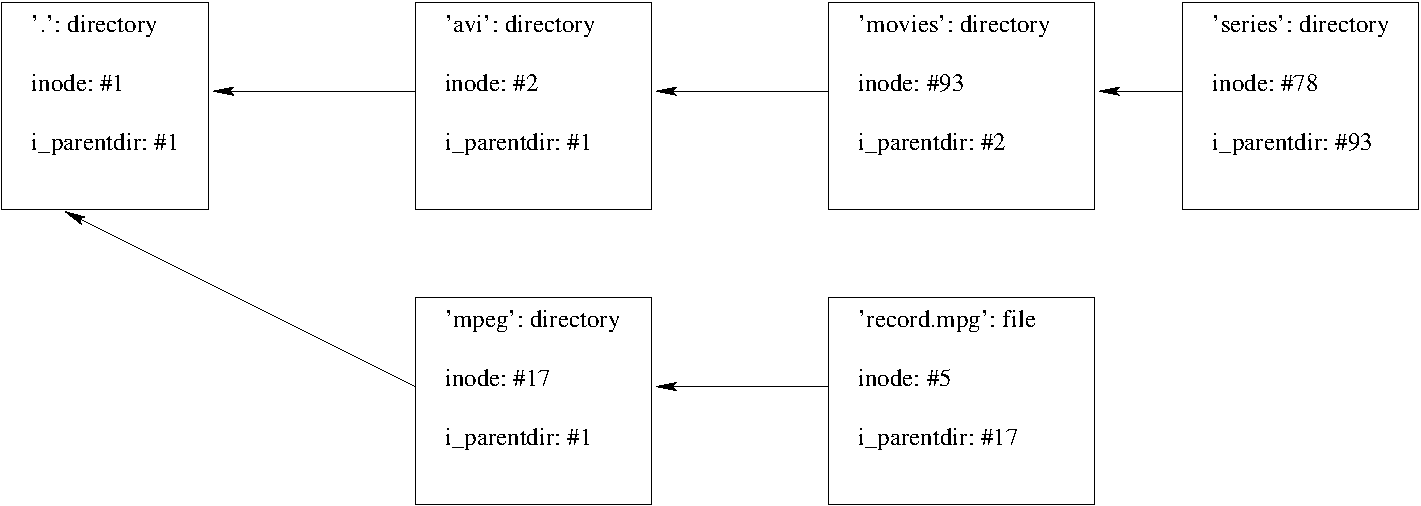
\includegraphics[height=5cm]{dir}
\caption{Nesting of directories}
\end{figure}

The tree for the figure is:

\begin{verbatim}
/
/avi
/avi/movies
/avi/movies/series
/mpeg
/mpeg/record.mpg
\end{verbatim}

\subsection{File Inode}
\label{fileinode}

An ordinary file, which contains data. The actual data blocks associated with the file are stored in \wi{extent} structures.

\index{struct!lime\_file\_inode}
\begin{verbatim}
#define LIME_EXTENTS_PER_INODE 80

struct lime_file_inode {
 uint32_t fi_boff;
 uint32_t fi_eoff;
 uint32_t fi_numextents;
 struct   lime_extent fi_extents[LIME_EXTENTS_PER_INODE];
};
\end{verbatim}

\begin{tabularx}{\textwidth}{|l|X|}
\hline
fi\_boff&Begin offset within the first extent \\
\hline
fi\_eoff&End offset within the last extent \\
\hline
fi\_numextents&Number of extents used \\
\hline
fi\_extents&Structure used to store the extents \\
\hline
\end{tabularx}

As stated in the definitions on page \pageref{defs}, an extent is simply a (offset, length) tuple. It contains the block offset, and the number of blocks used from this offset onwards.

\newpage

% let the text stand out a bit more
\standon{Fragmentation study}{fragmentation!study}

As can be seen, we allow a maximum of 80 extents per file. If more extents are needed than this maximum, the file cannot be expanded beyond the current size.

In order to determine how much of an issue this is, Ad Denissen and I created a small tool which simulates an extent-based 250GB filesystem with 4MB data blocks. It simulates writing 10.000 files sized between 500 and 5000MB. If a file does not fit, it will delete an existing one at random to take fragmentation into account. Finally, we refuse to allocate the last 5\% of the data blocks in order to decrease fragmentation\footnote{This value is based on some tests to determine an acceptable value}.

Plotting an overview of the number of fragments per file and the average fragmentation gives an interesting result:

\begin{center}
\begin{figure}[h]
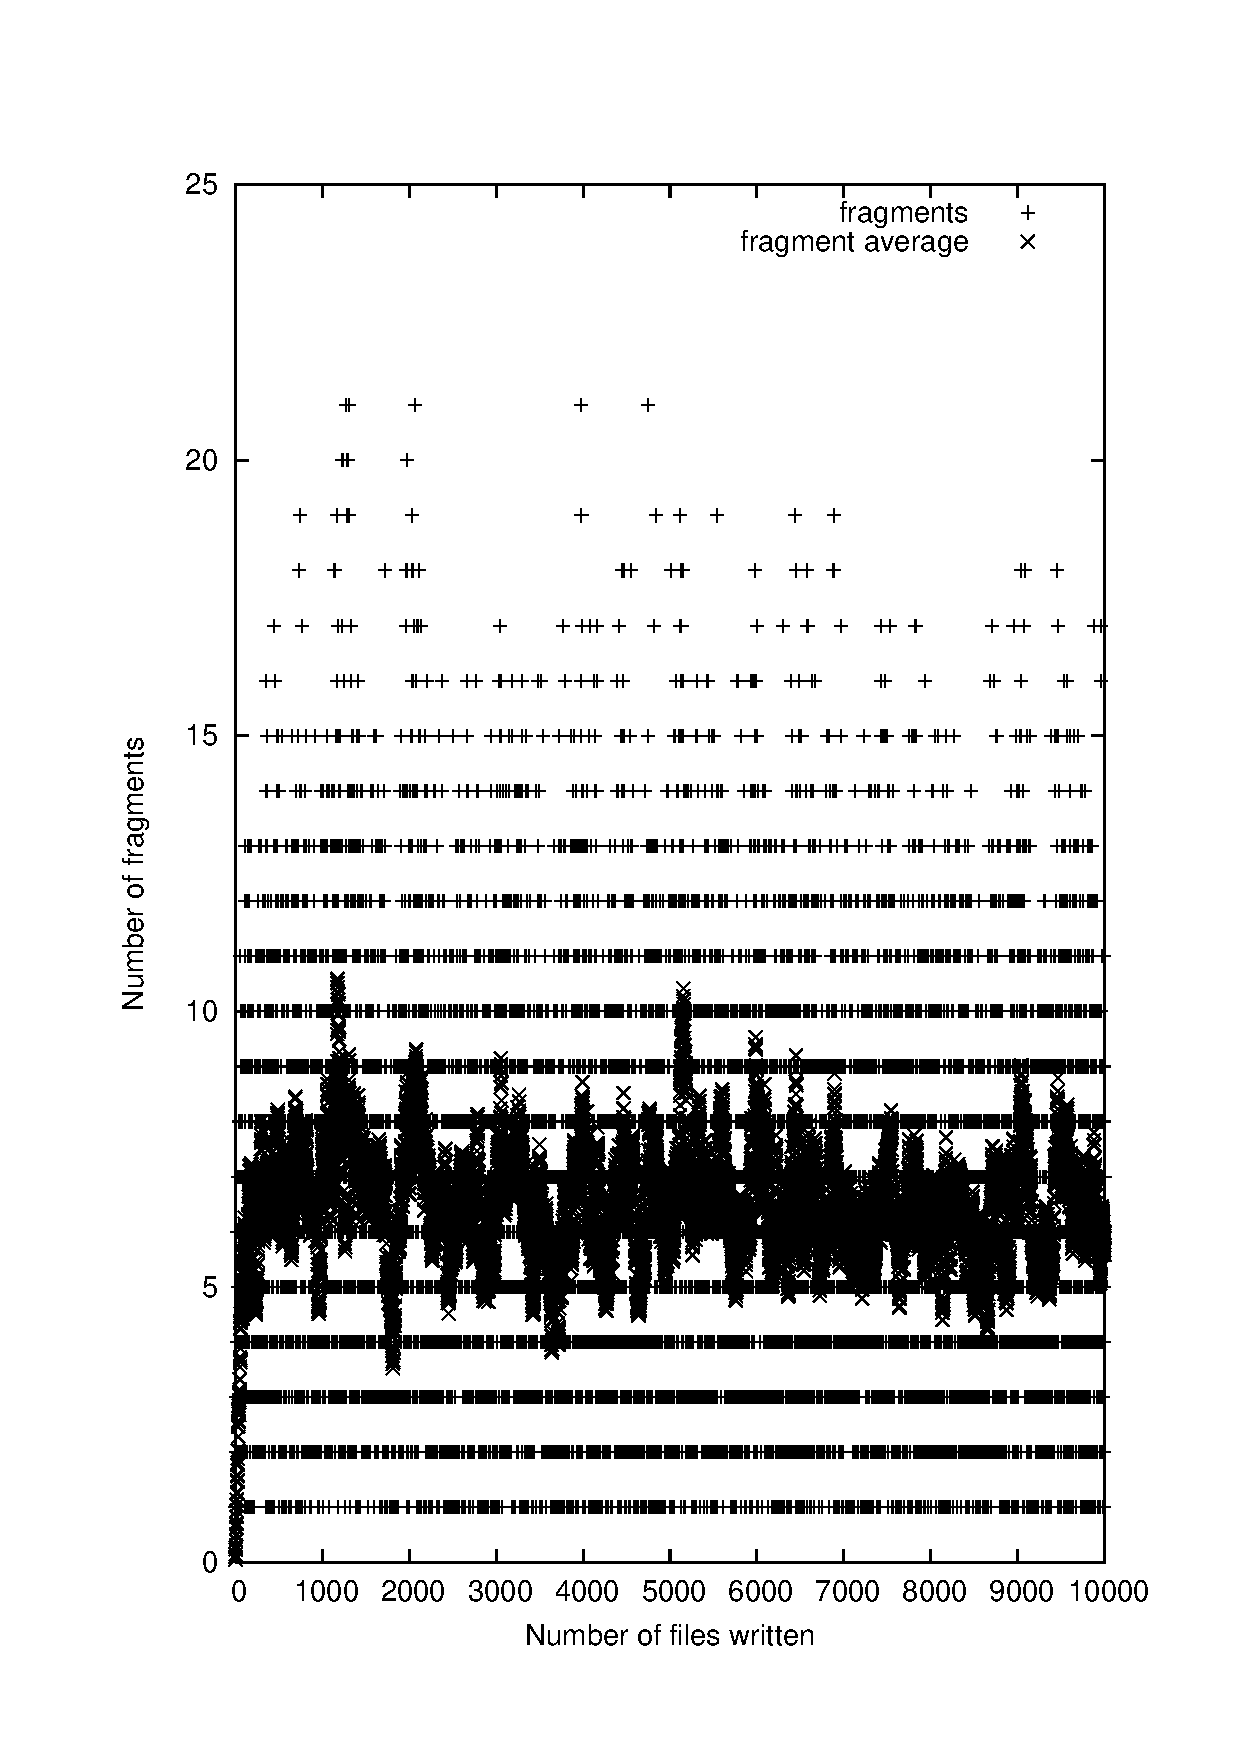
\includegraphics[width=7.5cm]{frag-log}
\caption{Fragments per file}
\end{figure}
\end{center}

As can be seen, the number of fragments never exceeds 21. This indicates the 80 extents we have is acceptable. However, it is also interesting to see the relationship between fragment sizes and the occurrence between them. 

In order to display this, we plot the fragment size as \emph{X} and the occurrence in \% as \emph{Y}. This gives the following result:

\begin{figure}[h]
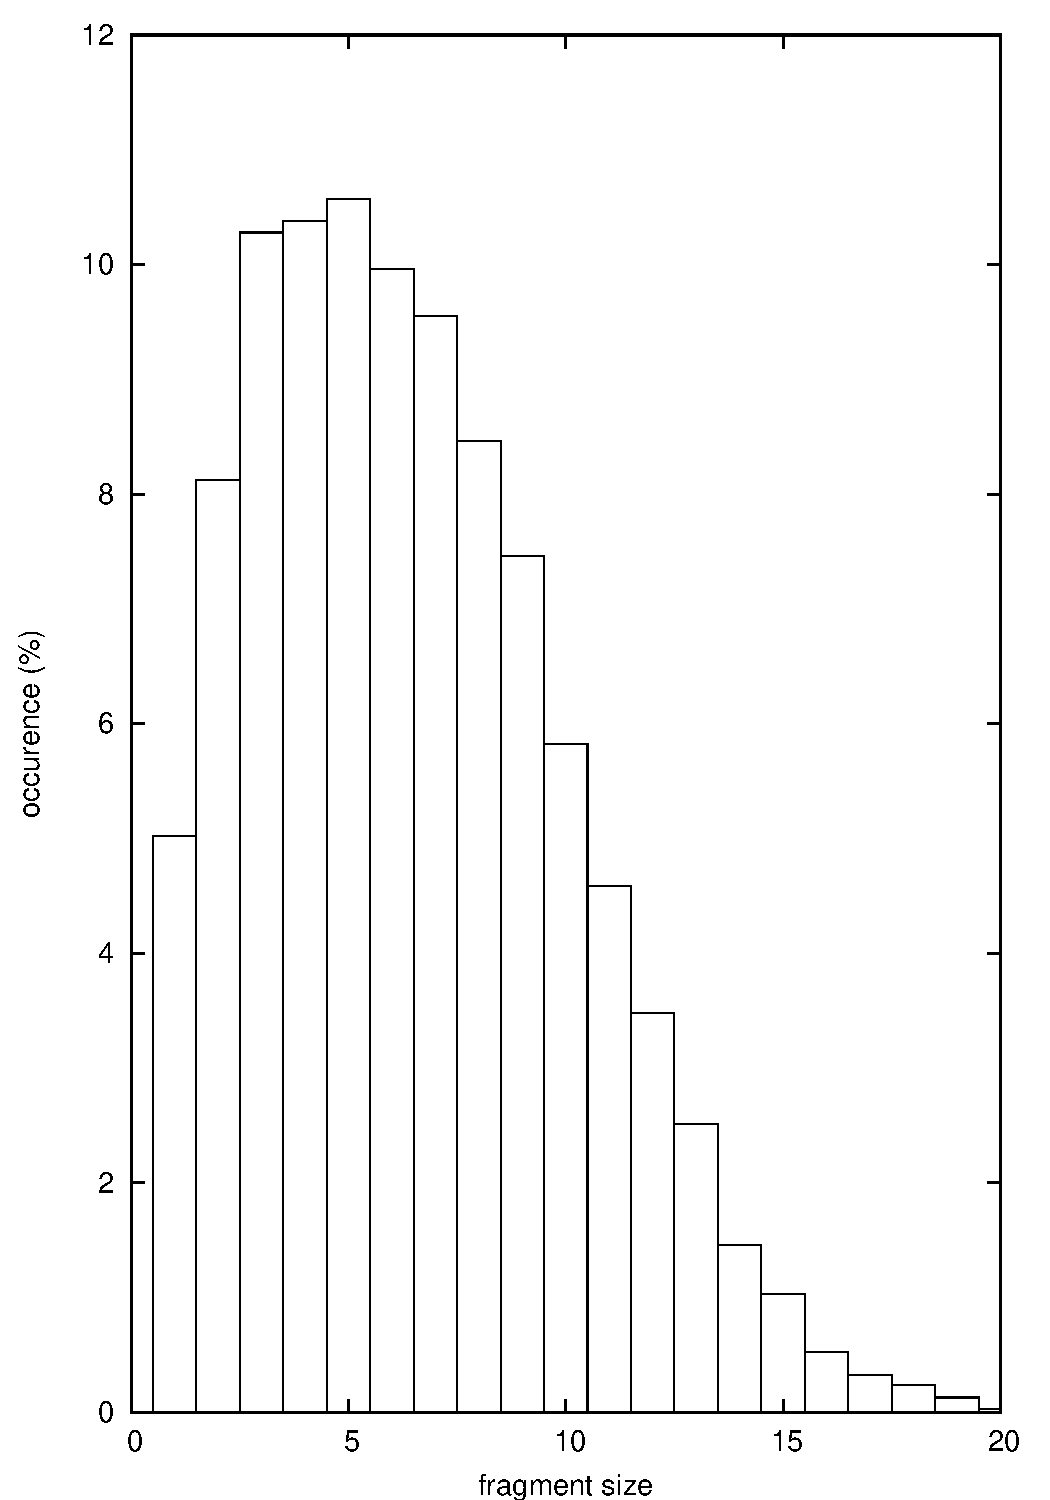
\includegraphics[width=7.5cm]{frag-occurence}
\caption{Fragment occurrence}
\end{figure}

As can be seen in these images, huge fragments are quite rare, even in everyday usage.

\standoff

The extent structure is defined as:

\index{struct!lime\_extent}
\begin{verbatim}
struct lime_extent {
 uint32_t ex_offset;
 uint32_t ex_length;
};
\end{verbatim}

Extents always point to the data blocks and will be expanded if more space is needed (refer to section \ref{allocation} for more information). There is a hard limit on how many extents a file can have (\texttt{LIME\_EXTENTS\_PER\_INODE}), therefore a file can always consist of a minimum of \\
$LIME\_EXTENDS\_PER\_INODE * sbBlockSize$ bytes.

As can be expected, the filesystem will always attempt to expand the last extent. More information about the block allocation can be found in section \ref{allocation} on page \pageref{allocation}. The figure below shows an example of extent administration:

\begin{figure}[h]
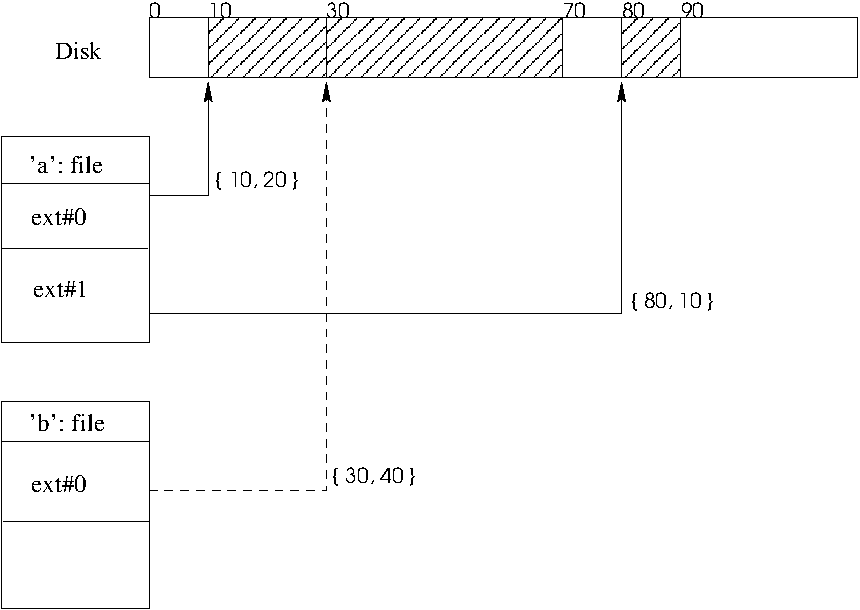
\includegraphics[width=10cm]{file-extent}
\caption{File-extent administration}
\end{figure}

\label{offs}As stated above, \texttt{boff} and \texttt{eoff} are offsets within the first and last block. Refer to the image below:

\begin{figure}[h]
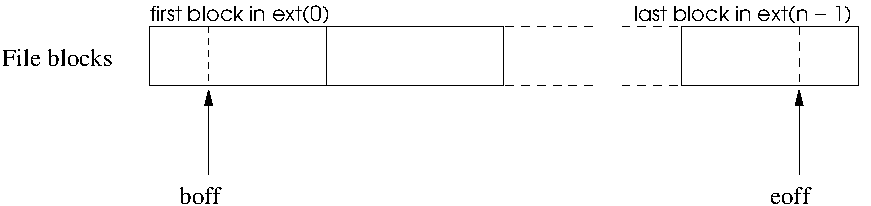
\includegraphics[width=10cm]{file-offs}
\caption{File begin- and end offsets}
\end{figure}

There are some implementation specific limitations on this approach, please refer to section \ref{impl_offs} for more information.

Based on these two offsets, the file size can be calculated in bytes as:

\begin{displaymath}
filesize = dataBlockSize \cdot \left( \sum_{i=0}^{n} ext(i)_{length} \right) - boff - \left( dataBlockSize - eoff \right)
\end{displaymath}

\subsection{Hardlink Inode}
\label{hardlink}

A \wi{hard link} is a reference to an inode, using a different name. Unlike traditional UNIX filesystems like FFS and ext, this filesystem allocates an extra inode with the hard link's name, but returns the destination inode. Therefore, we can implement this by simply storing the destination inode number.

\begin{figure}[h]
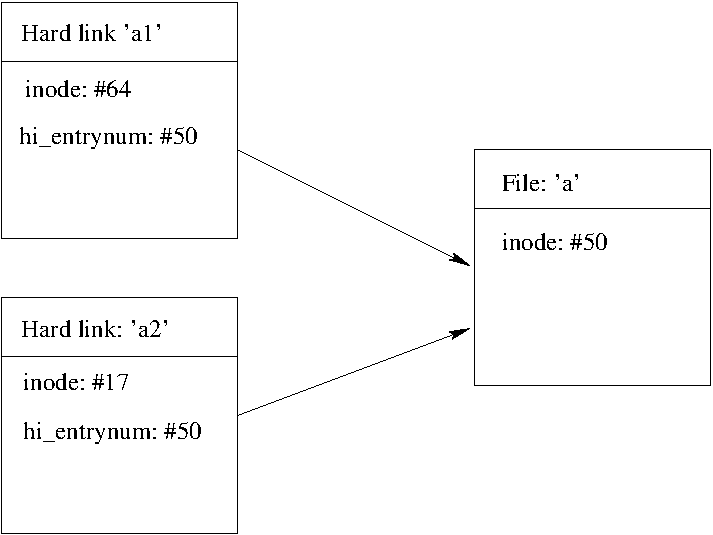
\includegraphics[height=5cm]{hard-link}
\caption{Hard link and file relationship}
\end{figure}
\index{struct!lime\_hlink\_inode}

\begin{verbatim}
struct lime_hlink_inode {
 uint32_t hi_entrynum;
};
\end{verbatim}

The implementation-specific notes can be found in section \ref{impl_hardlinks}.

\subsection{Softlink Inode}

A \wi{soft link}\footnote{also known as a symbolic link} is a reference to another location. It references by name, so therefore the destination doesn't have to be on this filesystem or even exist for that matter.

\index{struct!lime\_slink\_inode}
\begin{verbatim}
#define LIME_MAX_SYMLINK_LEN 256

struct lime_slink_inode {
 char si_path[LIME_MAX_SYMLINK_LEN];
};
\end{verbatim}

The soft link implementation is simple: all that needs to be done, is to pass the \texttt{si\_path} to the Linux VFS layer. This will resolve it to a new request to the accompanying filesystem.

\subsection{Checkpoint Inode}

The \wi{checkpoint inode} is used to determine the most recent copy of the FIT. It is always the final entry of the FIT; this increases the chance all entries are written before this final inode and thus are up-to-date.

\index{struct!lime\_checkpoint}
\begin{verbatim}
struct lime_checkpoint {
 uint32_t ci_followup;
};
\end{verbatim}

The followup count should only differ by 1, since they are used in a round-robin fashion. This means the FIT following the currently active FIT will be used. If the difference is not exactly one, the filesystem will not be mounted.

\section{Data blocks}

The data blocks start after the final File Allocation Table and are always aligned on a data block. They will continue until the end of the disk. The list of free blocks is constructed upon mount time, refer to section \ref{freespace} for more information.
